\documentclass[border=20pt, tikz]{standalone}
\usepackage{amsmath}
\usetikzlibrary{calc, arrows.meta, decorations.pathreplacing}

% =========================================================
% GLOBAL SETTINGS & COLORS
% =========================================================
\definecolor{colorX}{RGB}{239,68,68}       % Red
\definecolor{colorY}{RGB}{34,197,94}       % Green
\definecolor{colorZ}{RGB}{59,130,246}      % Blue
\definecolor{cornerCol}{RGB}{30,58,138}    % Dark Blue for corner coordinates

\tikzset{
    glass/.style={fill=cyan!15, draw=cyan!70!blue, thick, fill opacity=0.2, line join=round},
    axis/.style={thick, -{Latex[length=3mm, width=2mm]}},
    common settings/.style={
        font=\sffamily,
        x={(0.9cm, -0.15cm)}, 
        y={(0cm, 1cm)}, 
        z={(-0.6cm, -0.5cm)}
    }
}

\begin{document}

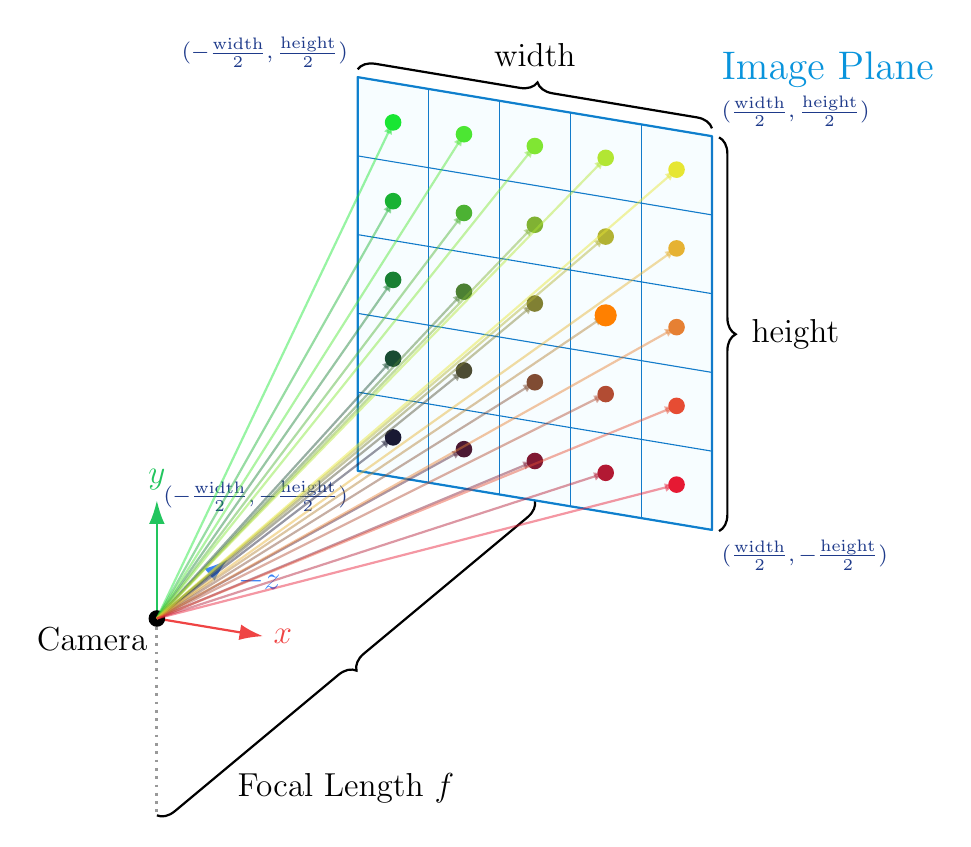
\begin{tikzpicture}[common settings, >=Stealth]

    % Configuration
    \def\zdist{8}      % Distance of image plane from camera
    \def\res{5}        % 5x5 resolution
    \def\pixSize{1.0}  % Size of each pixel
    \pgfmathsetmacro{\halfW}{(\res * \pixSize) / 2}

    % 1. Draw World / Camera Axes
    \draw[axis, colorX] (0,0,0) -- (1.5,0,0) node[right, font=\large] {$x$};
    \draw[axis, colorY] (0,0,0) -- (0,1.5,0) node[above, font=\large] {$y$};
    \draw[axis, colorZ] (0,0,0) -- (0,0,-1.5) node[below right, font=\large] {$-z$};
    
    \fill[black] (0,0,0) circle (3pt) node[below left, font=\large] {Camera};
    
    % Dotted line and focal length brace
    \draw[black, opacity=0.4, line width=1pt, dotted] (0,0,0) -- (0, -\halfW, 0);
    \draw[decorate, decoration={brace, amplitude=6pt, mirror}, thick]
        (0, -\halfW, 0) -- (0, -\halfW, -\zdist) 
        node[midway, below=38pt, font=\large] {Focal Length $f$};

    % 2. Draw Image Plane (Glass)
    \path[glass] (-\halfW, -\halfW, -\zdist) -- (\halfW, -\halfW, -\zdist) 
              -- (\halfW, \halfW, -\zdist) -- (-\halfW, \halfW, -\zdist) -- cycle;

    % Plane Label
    \node[cyan!80!blue, anchor=south west, font=\Large] at (\halfW, \halfW + 0.5, -\zdist) {Image Plane};

    % Width and Height braces
    \draw[decorate, decoration={brace, amplitude=6pt}, thick]
        (-\halfW, \halfW+0.1, -\zdist) -- (\halfW, \halfW+0.1, -\zdist) 
        node[midway, above=8pt, font=\large] {width};

    \draw[decorate, decoration={brace, amplitude=6pt, mirror}, thick]
        (\halfW+0.1, -\halfW, -\zdist) -- (\halfW+0.1, \halfW, -\zdist) 
        node[midway, right=8pt, font=\large] {height};

    % Corner Coordinate Bounds
    \node[anchor=south east, font=\footnotesize, cornerCol] at (-\halfW, \halfW, -\zdist) {$(-\frac{\text{width}}{2}, \frac{\text{height}}{2})$};
    \node[anchor=south west, font=\footnotesize, cornerCol] at (\halfW, \halfW, -\zdist) {$(\frac{\text{width}}{2}, \frac{\text{height}}{2})$};
    \node[anchor=north east, font=\footnotesize, cornerCol] at (-\halfW, -\halfW, -\zdist) {$(-\frac{\text{width}}{2}, -\frac{\text{height}}{2})$};
    \node[anchor=north west, font=\footnotesize, cornerCol] at (\halfW, -\halfW, -\zdist) {$(\frac{\text{width}}{2}, -\frac{\text{height}}{2})$};

    % 3. Draw 5x5 Grid Lines
    \foreach \i in {0,...,\res} {
        \pgfmathsetmacro{\pos}{-\halfW + \i * \pixSize}
        % Vertical lines
        \draw[cyan!60!blue, thin] (\pos, -\halfW, -\zdist) -- (\pos, \halfW, -\zdist);
        % Horizontal lines
        \draw[cyan!60!blue, thin] (-\halfW, \pos, -\zdist) -- (\halfW, \pos, -\zdist);
    }

    % 4. Generate Rays to Pixel Centers & Draw Colored Dots
    \foreach \ix in {0,...,4} {
        \foreach \iy in {0,...,4} {
            % Calculate pixel center coordinate (Y points UP in 3D physical space)
            \pgfmathsetmacro{\px}{-\halfW + (\ix + 0.5) * \pixSize}
            \pgfmathsetmacro{\py}{\halfW - (\iy + 0.5) * \pixSize}
            
            % Exact same color matching as the 2D steps
            \pgfmathsetmacro{\rcol}{0.1 + 0.8*(\ix/4)}
            \pgfmathsetmacro{\gcol}{0.1 + 0.8*((4 - \iy)/4)}
            \definecolor{pcol}{rgb}{\rcol, \gcol, 0.2}

            % Semi-transparent ray from camera to pixel
            \draw[pcol, opacity=0.45, line width=0.8pt, -{Latex[length=1.5mm]}] 
                 (0,0,0) -- (\px, \py, -\zdist);
            
            % Colored dot at the center of the pixel
            \fill[pcol] (\px, \py, -\zdist) circle (3pt);
        }
    }

    % 5. Highlight one specific "Primary Ray" for labeling
    % We target index (ix=3, iy=2) 
    \pgfmathsetmacro{\targetX}{-\halfW + (3 + 0.5) * \pixSize}
    \pgfmathsetmacro{\targetY}{\halfW - (2 + 0.5) * \pixSize}
    
    % Match the color of that specific ray
    \pgfmathsetmacro{\trcol}{0.1 + 0.8*(3/4)}
    \pgfmathsetmacro{\tgcol}{0.1 + 0.8*((4 - 2)/4)}
    \definecolor{targetCol}{rgb}{\trcol, \tgcol, 0.2}

    % % Draw solid highlighted ray
    % \draw[orange, line width=2pt, -{Latex[length=3.5mm]}] 
    %      (0,0,0) -- (\targetX, \targetY, -\zdist) 
    %      node[right=2pt, font=\Large, text=black, fill=white, fill opacity=0.85, text opacity=1, inner sep=3pt, rounded corners=2pt] {$\mathbf{d}_{ij}$};
    
    % Highlight its dot
    \fill[orange] (\targetX, \targetY, -\zdist) circle (4pt);

\end{tikzpicture}

\end{document}